\documentclass{article}

\usepackage{tikz}
\usetikzlibrary{shapes,backgrounds,intersections,positioning,calc,decorations.text,decorations.pathmorphing}

\pgfdeclarelayer{foreground}
%\pgfsetlayers{background}
\pgfsetlayers{main,foreground}

\begin{document}

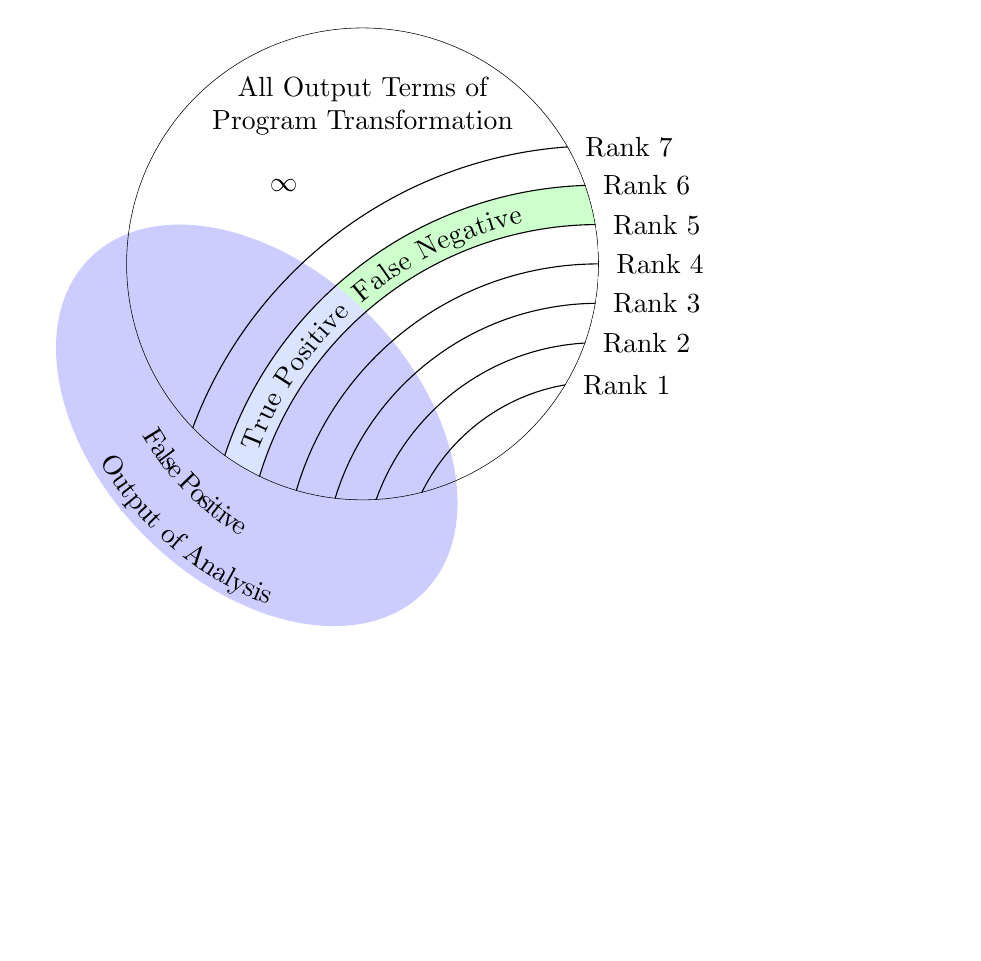
\begin{tikzpicture}[node distance=0.1cm]
  \begin{scope}[blend group=soft light, even odd rule]
    \fill[blue!20!white,rotate=45] (-2.4,-0.5) ellipse (2 and 3);
    \clip (0,0) circle (3);
    \clip (3,-4) circle (4.5) (-3,-3) rectangle (3,3);
    \fill[green!20!white] (3,-4) circle (5);
  \end{scope}

  \begin{pgfonlayer}{foreground}
    \path[decoration={text along path, text={False Negative}, text align={left indent=119ex}, transform={yshift=0.8ex}, reverse path},decorate] (3,-4) circle (4.5);
    \path[decoration={text along path, text={True Positive}, text align={left indent=104ex}, transform={yshift=0.8ex}, reverse path},decorate] (3,-4) circle (4.5);
    \draw[rotate=45,name path=output,decoration={text along path, text={Output of Analysis}, text align={left indent=45ex}, transform={yshift=0.8ex}},decorate] (-2.4,-0.5) ellipse (2 and 3);
    \path[rotate=45,name path=output,decoration={text along path, text={False Positive}, text align={left indent=45ex}, transform={yshift=5ex}},decorate] (-2.4,-0.5) ellipse (2 and 3);
    
    \clip (0,0) circle (3);
    \draw[name path=outer] (0,0) circle (3);
    \draw[name path=inner1] (3,-4) circle (2.5);
    \draw[name path=inner2]  (3,-4) circle (3);
    \draw[name path=inner3] (3,-4) circle (3.5);
    \draw[name path=inner4] (3,-4) circle (4);
    \draw[name path=inner5] (3,-4) circle (4.5);
    \draw[name path=inner6] (3,-4) circle (5);
    \draw[name path=inner7] (3,-4) circle (5.5);
    
    \path[name intersections={of=outer and inner1,name=rank1}];
    \path[name intersections={of=outer and inner2,name=rank2}];
    \path[name intersections={of=outer and inner3,name=rank3}];
    \path[name intersections={of=outer and inner4,name=rank4}];
    \path[name intersections={of=outer and inner5,name=rank5}];
    \path[name intersections={of=outer and inner6,name=rank6}];
    \path[name intersections={of=outer and inner7,name=rank7}];
  \end{pgfonlayer}

  \node[right=of rank1-1] {Rank 1};
  \node[right=of rank2-1] {Rank 2};
  \node[right=of rank3-2] {Rank 3};
  \node[right=of rank4-1] {Rank 4};
  \node[right=of rank5-1] {Rank 5};
  \node[right=of rank6-1] {Rank 6};
  \node[right=of rank7-1] {Rank 7};

  \node[align=center] at (0,2) {All Output Terms of \\ Program Transformation};
  \node at (-1,1) {$\infty$};
\end{tikzpicture}
\end{document}

%%% Local Variables:
%%% mode: latex
%%% TeX-master: t
%%% End:
